\documentclass{article}

% Allows to use functionalities related to images
\usepackage{graphicx}
% Allows to call a command that includes a bunch of extra text
% non-related to anything, just includes some randome text (not being
% meaninigless)
\usepackage{blindtext}
% Allows to set the location of a figure as pleased
\usepackage{wrapfig}
\author{Pablo Acereda}
\title{The Logic of Images and Figure in {\LaTeX}}

\begin{document}

\maketitle

Here is a new document.
%----------------------------------------------------------------------
\begin{center}
Sets manually its width and height
Keep maximum ratio so it doesn't get weird looking (not too little
height/ratio)

\includegraphics[width=5in,height=3in,keepaspectratio]{linux.png}
\end{center}
%----------------------------------------------------------------------

%----------------------------------------------------------------------
\begin{center}
Scales to half its size

\includegraphics[scale=0.5]{linux.png}
\end{center}
%----------------------------------------------------------------------

%----------------------------------------------------------------------
\begin{center}
Fits the whole line

\includegraphics[width=\textwidth]{linux.png}
\end{center}
%----------------------------------------------------------------------

%----------------------------------------------------------------------
\begin{center}
By writing a relation before the textwidth, the image shall be reduce to that
percentage of its size

\includegraphics[width=0.7\textwidth]{linux.png}
\end{center}
%----------------------------------------------------------------------

%----------------------------------------------------------------------
\begin{center}
Changes image's angle

\includegraphics[angle=90]{linux.png}
\end{center}
%----------------------------------------------------------------------

%Some random text------------------------------------------------------
\blindtext

% LaTeX puts figueres where it's more efficient: where they are most
% space-saving
% [h] will put the figure at the plave you wanted it to be
% [t] will put the figure at the top    of the page
% [b] will put the figure at the bottom of the page
% [p] will put the figure at a page of its own
\begin{figure}[h]
\centering

\includegraphics[width=0.7\textwidth]{emacs.jpg}
\caption{The effects of emacs on your fingers.}
\end{figure}

\blindtext

\blindtext

\blindtext

% Takes two arguments:
% 1 - Position
%     {r} Right
%     {l} Left
% 2 - How much do you want the image to take up
\begin{wrapfigure}{r}{3in}
\centering
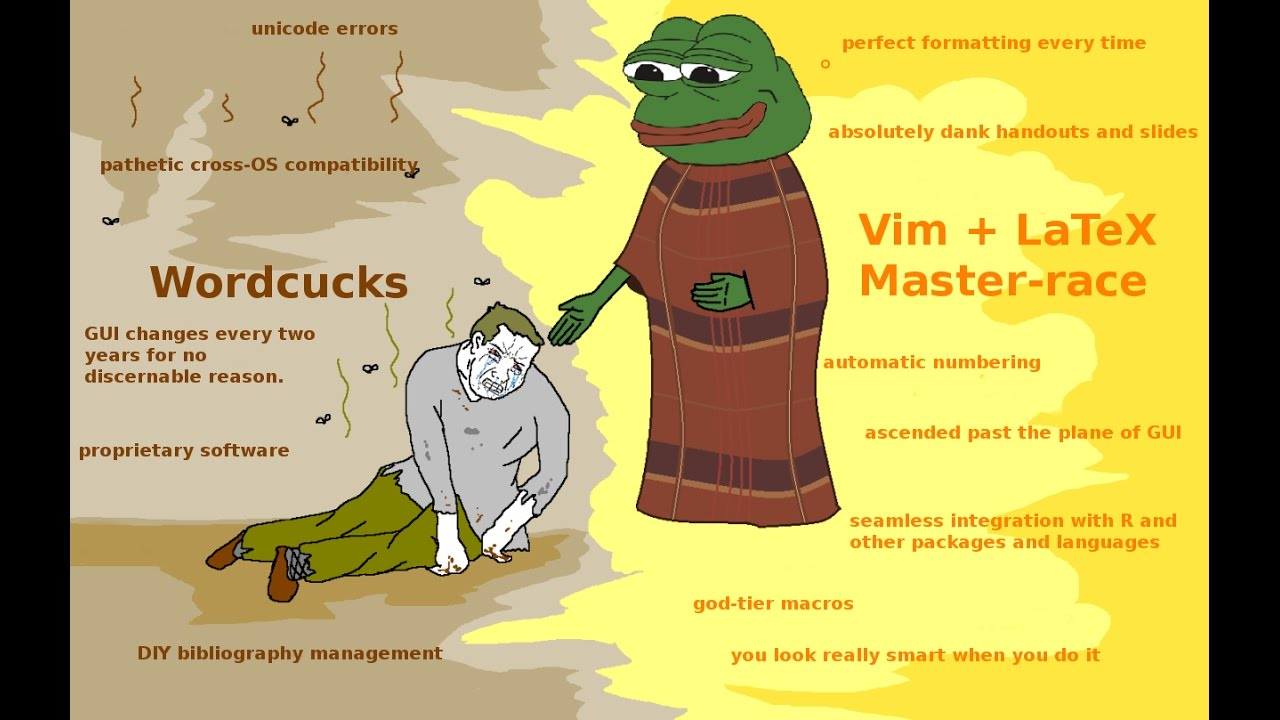
\includegraphics[width=2.5in]{vim_latex.jpg}
\caption{This is figure two\label{latexpic}}
\end{wrapfigure}

Please refer to Figure \ref{latexpic}.

\blindtext

\blindtext

\blindtext







\end{document}

